\documentclass[12pt, twoside]{article}
\usepackage[letterpaper, margin=1in, headsep=0.5in]{geometry}
\usepackage[english]{babel}
\usepackage[utf8]{inputenc}
\usepackage{amsmath}
\usepackage{amsfonts}
\usepackage{amssymb}
\usepackage{tikz}
\usetikzlibrary{quotes, angles}
\usepackage{graphicx}
\usepackage{enumitem}
\usepackage{multicol}
\usepackage{hyperref}

\newif\ifmeta
\metatrue %print standards and topics tags

\title{IB Mathematics}
\author{Chris Huson}
\date{February 2022}

\usepackage{fancyhdr}
\pagestyle{fancy}
\fancyhf{}
\renewcommand{\headrulewidth}{0pt} % disable the underline of the header
\raggedbottom


\fancyhead[LE]{\thepage}
\fancyhead[RO]{\thepage \\ Name: \hspace{4cm} \,\\}
\fancyhead[LO]{BECA / IB Math 4-Polynomial and rational functions \\* 11 February 2022}

\begin{document}

\subsubsection*{4.11 Exam: Polynomial and rational functions}
\begin{enumerate}
    \item Shown in the plot below is the function $f(x)=x^3-x^2-9x+9$.
    \begin{enumerate}
        \item Write down the value of $f(0)$. On the graph, mark the point for $f(0)$ with a star.\vspace{0.75cm}
        \item Write down the solutions to $f(x)=0$. Mark them with ``X'' marks on the graph.\vspace{0.75cm}
        \item Mark the portion of the function that is \emph{decreasing} with a squiggly line.
        \item Label the local maximum and local minimum as ordered pairs.
        \item Show that $1$ is an $x$-intercept because $x=1$ is a solution to $f(x)=0$.
    \end{enumerate}
    \begin{center}
        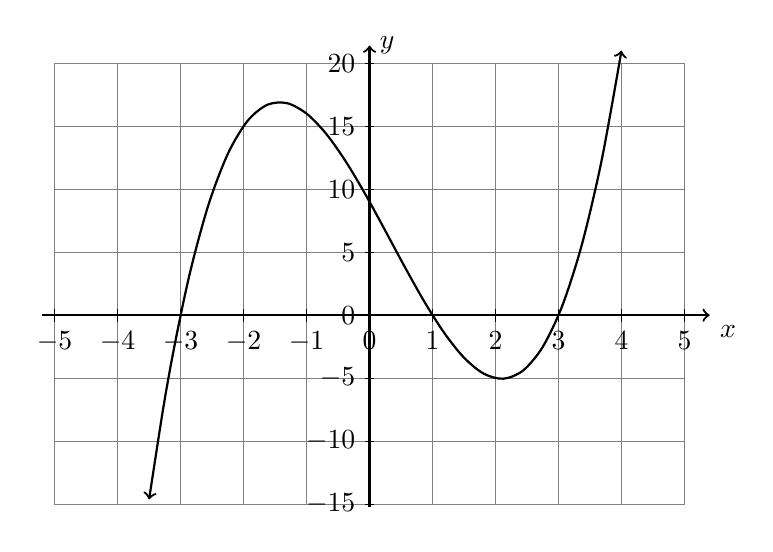
\begin{tikzpicture}[x=1cm, y=0.20cm, scale=0.8]
            \draw [help lines] (-5,-15.1) grid (5,20);
            \draw [thick, ->] (-5.2,0) -- (5.4,0) node [below right] {$x$};
            \draw [thick, ->] (0,-15.2)--(0,21.4) node [right] {$y$};
            \foreach \x in {-5,...,5}
                \draw[shift={(\x,0)}] (0,3pt)--(0,-3pt) node[below] {$\x$};
            \foreach \y in {-15,-10,...,20}
                \draw[shift={(0,\y)}] (2pt,0pt)--(-2pt,0pt) node[left]  {$\y$};
            \draw [<->,thick,smooth,domain=-3.5:4] plot(\x,{(\x)^3-(\x)^2-9*(\x)+9});
        \end{tikzpicture}
    \end{center}

\item A function composed of four points $\{ (-2,1),(j,1),(3,4),(5,k) \}$ is plotted on the below.
    \begin{multicols}{2}
    \begin{enumerate}
      \item Write down $j$
      \item Write down $k$
      \item Write down the domain.\vspace{0.5cm}
      \item Add an ordered pair to the relation so that it would \emph{not} be a function.
    \end{enumerate}
      \begin{center}
      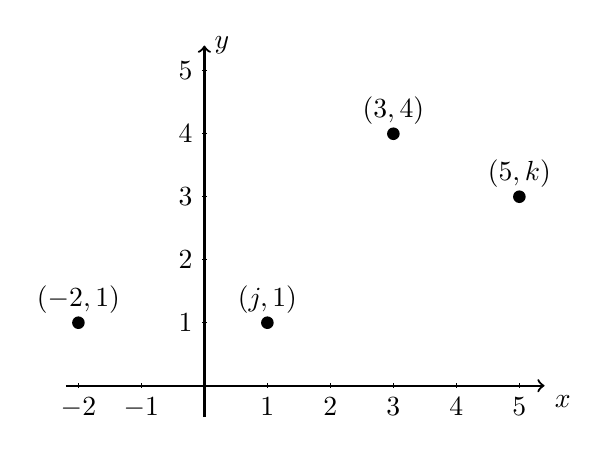
\begin{tikzpicture}[scale=0.8]
        %\draw [help lines] (-3,-2) grid (4,6);
        \draw [thick, ->] (-2.2,0) -- (5.4,0) node [below right] {$x$};
        \draw [thick, ->] (0,-0.5)--(0,5.4) node [right] {$y$};
        \foreach \x in {-2,-1,1,2,..., 5} \draw (\x cm,1pt) -- (\x cm,-1pt) node[anchor=north] {$\x$};
        \foreach \y in {1, 2, 3, 4, 5} \draw (1pt,\y cm) -- (-1pt,\y cm) node[anchor=east] {$\y$};
        %\draw [thick, <->] (-3.5,-1.5) -- (4.2,6.2);
        \fill (-2,1) circle[radius=0.1] node[above]{$(-2,1)$};
        \fill (1,1) circle[radius=0.1] node[above]{$(j,1)$};
        \fill (3,4) circle[radius=0.1] node[above]{$(3,4)$};
        \fill (5,3) circle[radius=0.1] node[above]{$(5,k)$};
      \end{tikzpicture}
      \end{center}
    \end{multicols}

\newpage

\item Plot the function $h(x)=x^{3}+x^{2}-6x$, labeling the $x-$ and $y$-intercepts. Mark the local maximum and minimums as ordered pairs.
    \begin{center}
        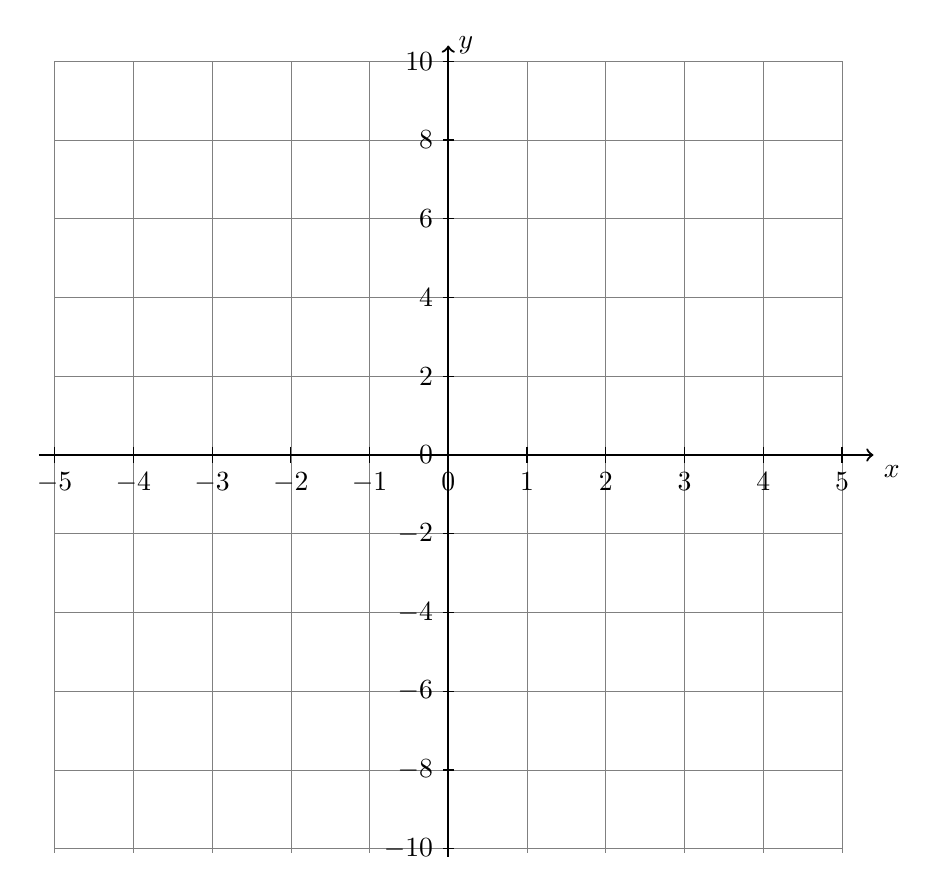
\begin{tikzpicture}[x=1cm, y=0.5cm]
            \draw [help lines] (-5,-10.1) grid (5,10);
            \draw [thick, ->] (-5.2,0) -- (5.4,0) node [below right] {$x$};
            \draw [thick, ->] (0,-10.2)--(0,10.4) node [right] {$y$};
            \foreach \x in {-5,...,5}
                \draw[shift={(\x,0)}] (0,3pt)--(0,-3pt) node[below] {$\x$};
            \foreach \y in {-10,-8,...,10}
                \draw[shift={(0,\y)}] (2pt,0pt)--(-2pt,0pt) node[left]  {$\y$};
            %\draw [<->,thick,smooth,domain=-3.5:2.5] plot(\x,{(\x)^3+(\x)^2-6*(\x)});
        \end{tikzpicture}
    \end{center}

\item The function $f(x)=ax^2+bx+c$ is graphed below over its domain, $p\leq x < q$.
    \begin{multicols}{2}
    \begin{enumerate}
      \item Write down the value of $c$.
      \item Write down $f(-1)$.
      \item Find $x$ such that $f(x)=6$.
      \item Write down the values of $p$, $q$.
      \item Write down the range of $f$. \vspace{1cm}
    \end{enumerate}
      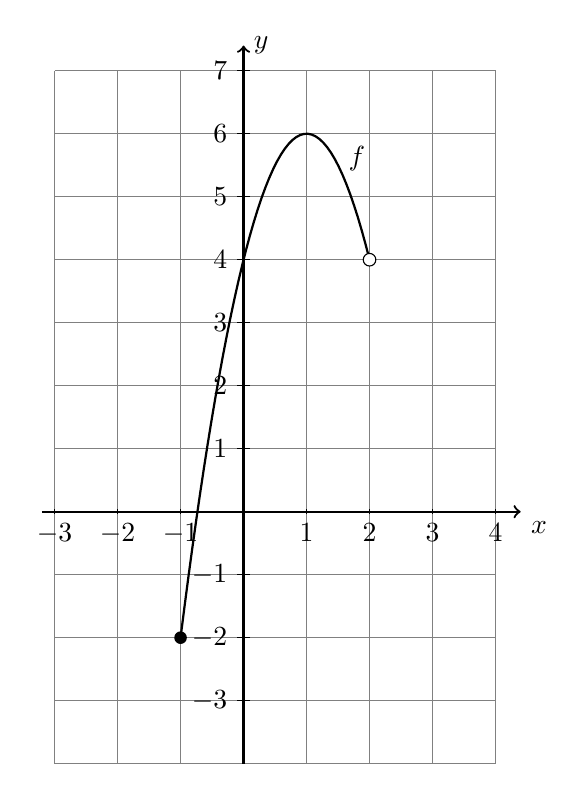
\begin{tikzpicture}[scale=0.8]
        \draw [help lines] (-3,-4) grid (4,7);
        \draw [thick, ->] (-3.2,0) -- (4.4,0) node [below right] {$x$};
        \draw [thick, ->] (0,-4)--(0,7.4) node [right] {$y$};
        \foreach \x in {-3,-2,-1,1,2, ..., 4} \draw (\x cm,1pt) -- (\x cm,-1pt) node[below] {$\x$};
        \foreach \y in {-3,-2,-1,1,2,...,7} \draw (3pt,\y cm) -- (-3pt,\y cm) node[left] {$\y$};
        \draw [thick,samples=50,domain=-1:2] plot(\x,-2*\x*\x+4*\x+4);
        \fill (-1,-2) circle[radius=0.1];
        \node at (1.8,5.6){$f$};
        \fill [white] (2,4) circle[radius=0.1];
        \draw (2,4) circle[radius=0.1];
      \end{tikzpicture}
    \end{multicols}
    \vspace{0.5cm}


    \newpage
    \item A ski jump is modeled by the cubic function $h(x)=1.0+0.7x+0.8x^2-0.35x^{3}$ where $h$ is the height in meters above ground and $x$ is the horizontal distance (m).
    \begin{multicols}{2}
        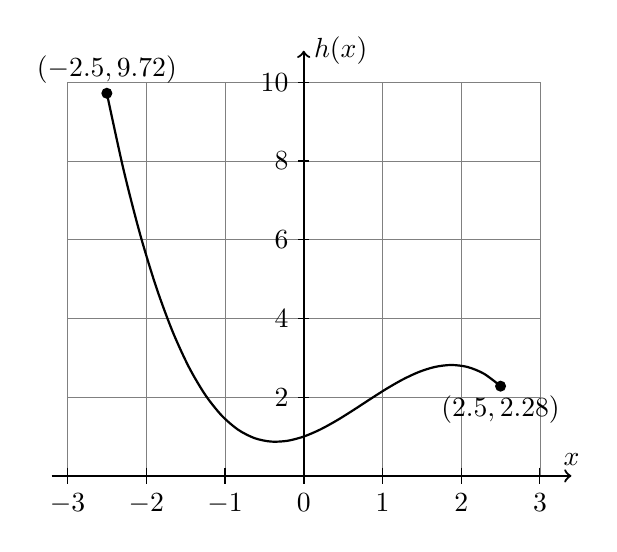
\begin{tikzpicture}[x=1cm, y=0.5cm, scale=1]
            \draw [help lines] (-3,0) grid (3,10);
            \draw [thick, ->] (-3.2,0) -- (3.4,0) node [above] {$x$};
            \draw [thick, ->] (0,-0.2)--(0,10.8) node [right] {$h(x)$};
            \foreach \x in {-3,...,3}
                \draw[shift={(\x,0)}] (0,3pt)--(0,-3pt) node[below] {$\x$};
            \foreach \y in {2,4,...,10}
                \draw[shift={(0,\y)}] (2pt,0pt)--(-2pt,0pt) node[left]  {$\y$};
            \draw [-,thick,smooth,domain=-2.5:2.5] plot(\x,{-0.35*(\x)^3+0.8*(\x)^2+0.7*(\x)+1});
            \fill (-2.5,9.72) ellipse(2pt and 2pt) node [above]{$(-2.5,9.72)$};
            \fill (2.5,2.28) ellipse(2pt and 2pt) node [below]{$(2.5,2.28)$};
        \end{tikzpicture}
        \begin{enumerate}[itemsep=0.5cm]
            \item The two ends of the ramp are marked as ordered pairs. How wide is the ramp in meters?
            \item What is the total vertical descent from the top of the ramp to its lowest point? \vspace{1cm}\\ \, %answer 8.85m
        \end{enumerate} 
        \end{multicols}

    \item Given two functions, a quadratic function $f(x)=0.6x^2+2.1x-3$ and a linear function $g(x)=1.2x+2$.
    \begin{enumerate}%[itemsep=1cm]
        \item Graph the parabola $y=f(x)$, marking the $y$-intercept and the vertex as an ordered pair.
        \item Find the coordinates of the two intercepts with the $x$-axis, the roots or zeros of $f(x)$.\vspace{1cm}
        \item Plot the linear function, $y=g(x)$. Mark and label the two intersections of the two functions $f(x)=g(x)$ as ordered pairs. Round to the nearest hundredth.
    \end{enumerate}
    \begin{center}
    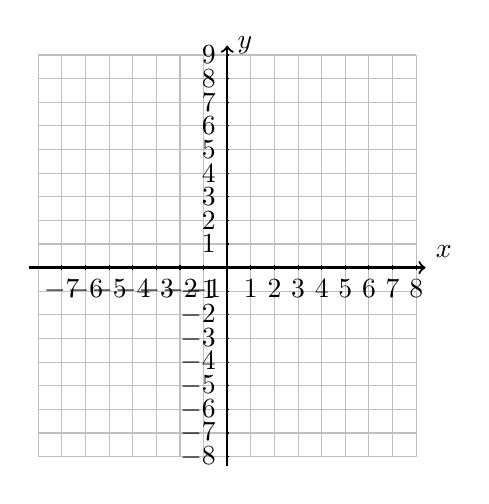
\begin{tikzpicture}[scale=0.3]
        \draw [thin, color=lightgray,, xstep=1.0cm,ystep=1.0cm] (-8,-8) grid (8,9);
        \foreach \x in {-7,...,-1,1,2,...,8}
        \draw (\x cm,3pt) -- (\x cm,-3pt) node[below] {$\x$};
        \foreach \y in {-8,...,-1,1,2,...,9}
        \draw[shift={(0,\y)},color=black] (2pt,0pt) -- (-2pt,0pt) node[left]  {$\y$};
        \draw [thick, ->] (-8.4,0) -- (+8.4,0) node [above right] {$x$};
        \draw [thick, ->] (0,-8.4) -- (0,9.4) node [right] {$y$};
        %\draw [thick, <->,smooth,domain=-5:2] plot(\x,0.6*\x*\x+2.1*\x-3);
        %\draw [thick, <->,smooth,domain=-5:2] plot(\x,1.2*\x+2);
    \end{tikzpicture}
    \end{center}

\newpage    
\item A rational function of the form $\displaystyle f(x)=\frac{1}{x-p}+q$ is shown on the grid below. 
    \begin{multicols}{2}
        \begin{enumerate}[itemsep=0.7cm]
            \item Write down the equation of the horizontal asymptote.
            \item  Write down the equation of the vertical asymptote.
            \item Hence, write down $p$ and $q$.
            \item Find $f(0)$.
            \item Solve for $x$ such that $f(x)=0$. \vspace{1cm} \\ \,
        \end{enumerate}
        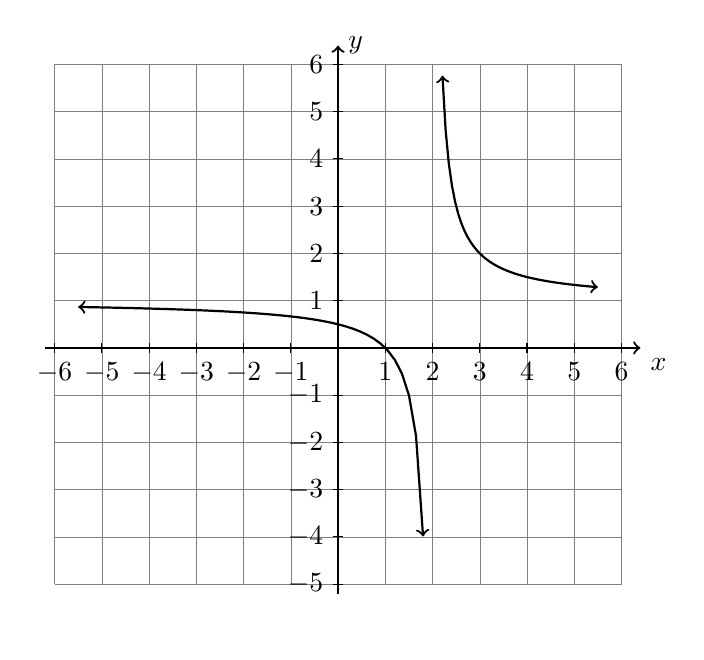
\begin{tikzpicture}[scale=0.6]
        \draw [help lines] (-6,-5) grid (6,6);
        \draw [thick, ->] (-6.2,0) -- (6.4,0) node [below right] {$x$};
        \draw [thick, ->] (0,-5.2)--(0,6.4) node [right] {$y$};
        \foreach \x in {-6,...,-3,-2,-1,1,2,...,6} \draw (\x cm,3pt) -- (\x cm,-3pt) node[below] {$\x$};
        \foreach \y in {-5,...,-3,-2,-1,1,2,...,6} \draw (3pt,\y cm) -- (-3pt,\y cm) node[left] {$\y$};
        \clip (-6,-6) rectangle (6,6);
        \draw [<->,thick,samples=50,domain=-5.5:1.8] plot(\x,{1/(\x-2)+1});
        \draw [<->,thick,samples=50,domain=2.21:5.5] plot(\x,{1/(\x-2)+1});
        \end{tikzpicture}
    \end{multicols}

\item The temperature ($C^\circ$) over a 24 hour day starting at midnight is modeled by the function $f\left(t\right)=-0.0063t^{3}+0.12t^{2}+0.38t+9$.
    \begin{enumerate}[itemsep=1cm]
        \item Write down the temperature at midnight, when $t=0$.
        \item Over what interval is the temperature increasing?
        \item Find the maximum temperature during the day.  \vspace{1cm}
    \end{enumerate}
    \begin{center}
    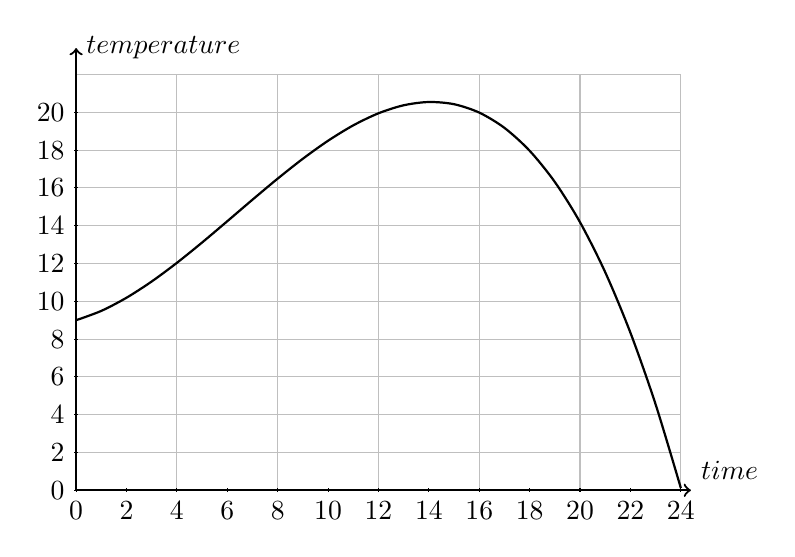
\begin{tikzpicture}[xscale=0.4, yscale=0.3, scale=0.8]
        \draw [thin, color=lightgray, xstep=4.0cm,ystep=2.0cm] (0,0) grid (24,22);
        \foreach \x in {0,2,...,24}
        \draw (\x cm,3pt) -- (\x cm,-3pt) node[below] {$\x$};
        \foreach \y in {0,2,...,20}
        \draw[shift={(0,\y)},color=black] (2pt,0pt) -- (-2pt,0pt) node[left]{$\y$};
        \draw [thick, ->] (0,0) -- (+24.4,0) node [above right]{$time$};
        \draw [thick, ->] (0,0) -- (0,23.4) node [right]{$temperature$};
        \draw [thick, smooth,domain=0.:24] plot(\x,-0.0063*\x*\x*\x+0.12*\x*\x+0.38*\x+9);
    \end{tikzpicture}
    \end{center}

\newpage
\subsubsection*{Linear functions}
\item A linear function $f$ is graphed below.
    \begin{multicols}{2}
    \begin{enumerate}
      \item Write down it's slope.\\ $m=$
      \vspace{0.25cm}
      \item Write down it's $y$-intercept.\\ $b=$
      \vspace{0.25cm}
      \item Write down the equation of the line.
    \end{enumerate} \vspace{.5cm}
      \begin{center} 
      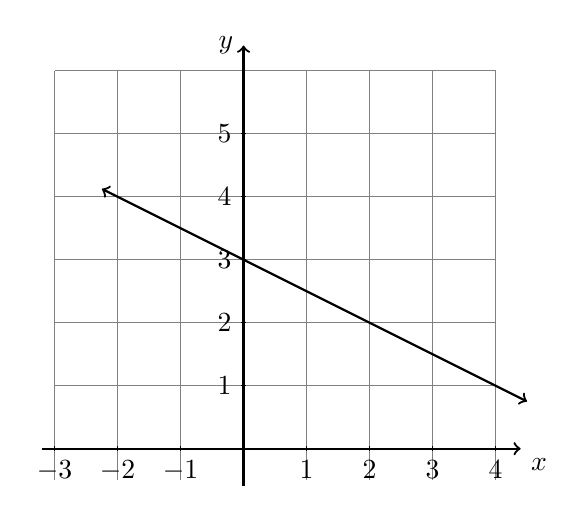
\begin{tikzpicture}[scale=0.8]
        \draw [help lines] (-3,-0.5) grid (4,6);
        \draw [thick, ->] (-3.2,0) -- (4.4,0) node [below right] {$x$};
        \draw [thick, ->] (0,-0.6)--(0,6.4) node [left] {$y$};
        \foreach \x in {-3,-2,-1,1,2,...,4} \draw (\x cm,1pt) -- (\x cm,-1pt) node[anchor=north] {$\x$};
        \foreach \y in {1, 2, 3, 4, 5} \draw (1pt,\y cm) -- (-1pt,\y cm) node[anchor=east] {$\y$};
        \draw [thick, <->,smooth,samples=20,domain=-2.25:4.5] plot(\x,-0.5*\x+3);
      \end{tikzpicture}
      \end{center}
    \end{multicols} \vspace{1cm}
    
    \item Write the linear equation $y+1=2(x-6)$ in the form $y=mx+c$. \vspace{4cm}
    
    \item A line has a gradient (slope) of $\displaystyle -\frac{3}{2}$ and passes through the point $(6, 1)$. Find the equation of the line in the form $y=mx+c$.
    
\newpage
\item A line goes through the points $(2,3)$ and $(6, -1)$. \hfill [5]
    \begin{enumerate}
      \begin{multicols}{2}
          \item Find the gradient of the line.
          \item Find the equation of the line in the form $y=mx+c$.\vspace{2cm}
          \begin{center}
          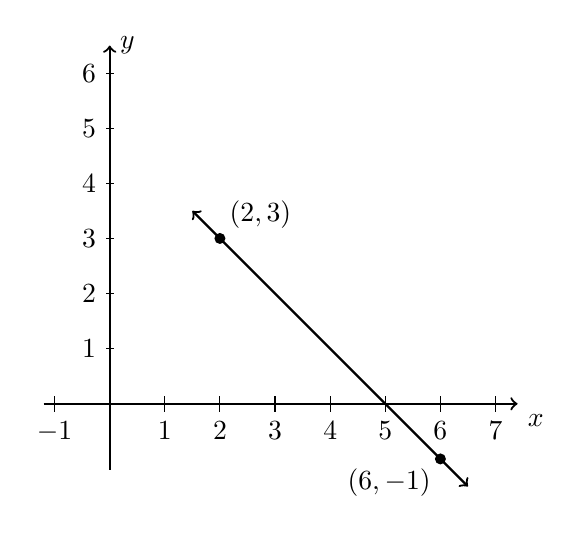
\begin{tikzpicture}[xscale=0.7, yscale=0.7]
            %\draw [help lines] (-3,-2) grid (4,6);
            \draw [thick, ->] (-1.2,0) -- (7.4,0) node [below right] {$x$};
            \draw [thick, ->] (0,-1.2)--(0,6.5) node [right] {$y$};
            \foreach \x in {-1, 1,2, ...,7} \draw (\x cm,4pt) -- (\x cm,-4pt) node[anchor=north] {$\x$};
            \foreach \y in {1,2,...,6} \draw (2pt,\y cm) -- (-2pt,\y cm) node[anchor=east] {$\y$};
            \fill (2,3) circle[radius=0.1] node[above right]{$(2,3)$};
            \fill (6,-1) circle[radius=0.1] node[below left]{$(6,-1)$};
            \draw [thick, <->,smooth,samples=20,domain=1.5:6.5] plot(\x,-1.0*\x+5);
          \end{tikzpicture}
          \end{center}
        \end{multicols}
    \end{enumerate} \vspace{2.cm}
    
\item A linear equation is desired to model a set of data.
\begin{enumerate}
    \item Plot the following points on the grid: $(-4,2)$, $(-3,1)$, $(-1,2)$, $(1,4)$, $(3,5)$, $(5,5)$
    \item Draw a line of best fit through the data. (use a straight edge for full credit)
    \item Write down the equation of the line.
\end{enumerate}
    \begin{center}
        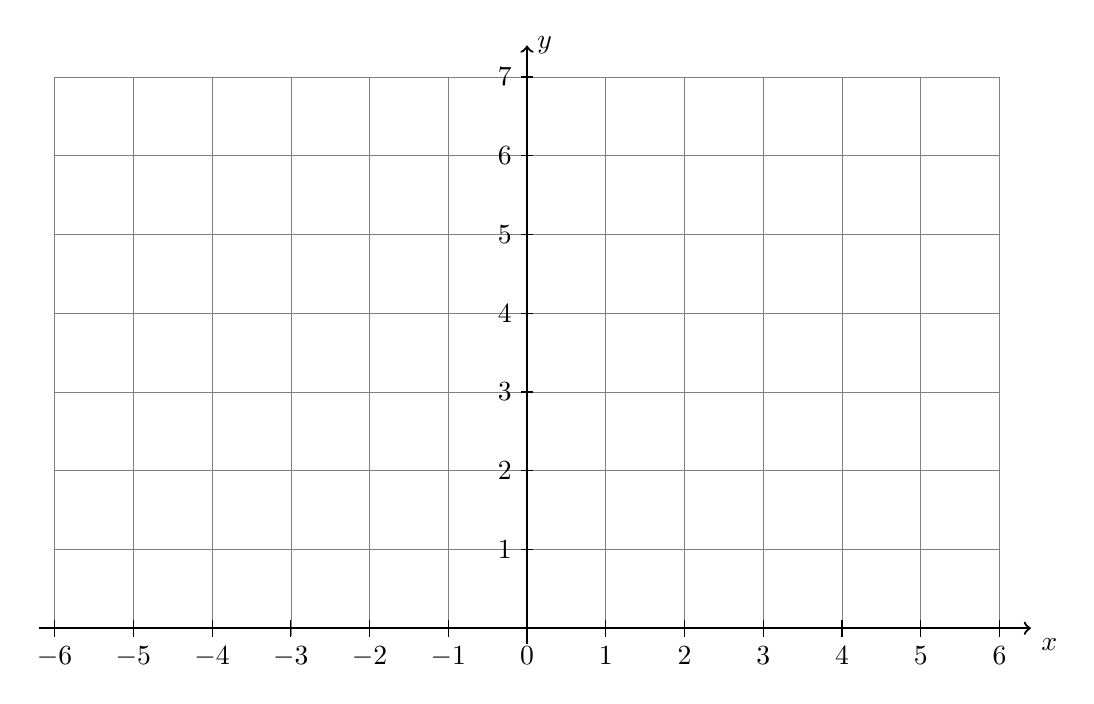
\begin{tikzpicture}[x=1cm, y=1cm, scale=1]
            \draw [help lines] (-6,-0.1) grid (6,7);
            \draw [thick, ->] (-6.2,0) -- (6.4,0) node [below right] {$x$};
            \draw [thick, ->] (0,-0.2)--(0,7.4) node [right] {$y$};
            \foreach \x in {-6,...,6}
                \draw[shift={(\x,0)}] (0,3pt)--(0,-3pt) node[below] {$\x$};
            \foreach \y in {1,...,7}
                \draw[shift={(0,\y)}] (2pt,0pt)--(-2pt,0pt) node[left]  {$\y$};
            \clip (-5,0) rectangle (5,5);
            %\draw [<->,thick,smooth,domain=-5:5] plot(\x,{(\x)^3+-4*(\x)^2-1*(\x)+4});
        \end{tikzpicture}
    \end{center}


\end{enumerate}
\end{document}



